\chapter{Analisi dei requisiti}
\label{cap:analisi-requisiti}

\intro{Il seguente capitolo assume la funzione di illustrare i casi d'uso e i requisiti raccolti nella fase di analisi del progetto commissionato.}

\setlength{\parskip}{3ex}

\section{Casi d'uso}
Per poter capire e studiare a fondo tutte le funzionalità che devono essere messe a disposizione dell'utente che utilizza l'applicativo da sviluppare, sono stati realizzati i relativi diagrammi dei casi d'uso di tipo UML. Tali diagrammi sono risultati fondamentali per individuare correttamente tutti i requisiti del sistema in questione.

\setlength{\parskip}{3ex}

\noindent Ciascun caso d'uso è costituito da:
\begin{itemize}
\item attore primario;
\item precondizione;
\item postcondizione;
\item scenario principale;
\item estensioni (qualora fossero presenti).
\end{itemize}

\setlength{\parskip}{3ex}

\noindent I casi d'uso identificati dalla sigla "UCE" rappresentano un caso d'uso d'errore.
L'unico attore coinvolto e identificato come \textit{Utente autenticato} corrisponde ad un qualunque dipendente dell'area commerciale di CWBI, al quale sono stati assegnati i permessi necessari a svolgere le operazioni di seguito riportate.  

\pagebreak

\subsection{UC0: Menu}
\begin{figure}[!h]
\centering
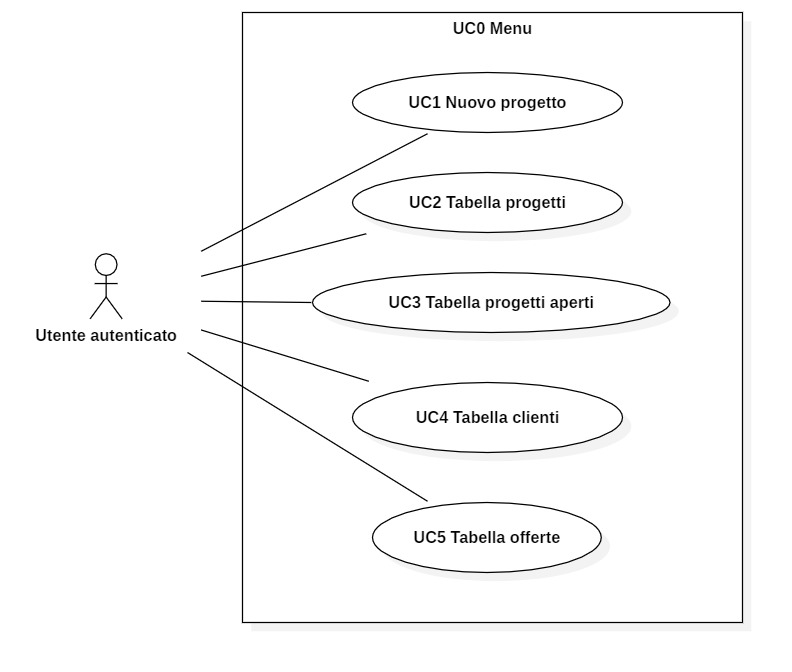
\includegraphics[width=300px]{../images/UC/.jpeg/UC0-menu.jpg}
\caption{UC0: Menu}
\end{figure}

\begin{itemize}
\item \textbf{Attore primario}: Utente autenticato.
\item \textbf{Precondizione}: L'attore ha accesso al modulo \textit{Campaign} della webapp CW GEST.
\item \textbf{Postcondizione}: Il sistema è pronto all'uso.
\item \textbf{Scenario principale}: 
\begin{enumerate}
\item L'attore crea un nuovo progetto [UC1].
\item L'attore accede alla tabella dei progetti [UC2].
\item L'attore accede alla tabella dei progetti aperti [UC3].
\item L'attore accede alla tabella dei clienti [UC4].
\item L'attore accede alla tabella delle offerte [UC5].
\end{enumerate}
\end{itemize}

\pagebreak

\subsection{UC1: Crea-Modifica progetto}
\begin{figure}[!h]
\centering
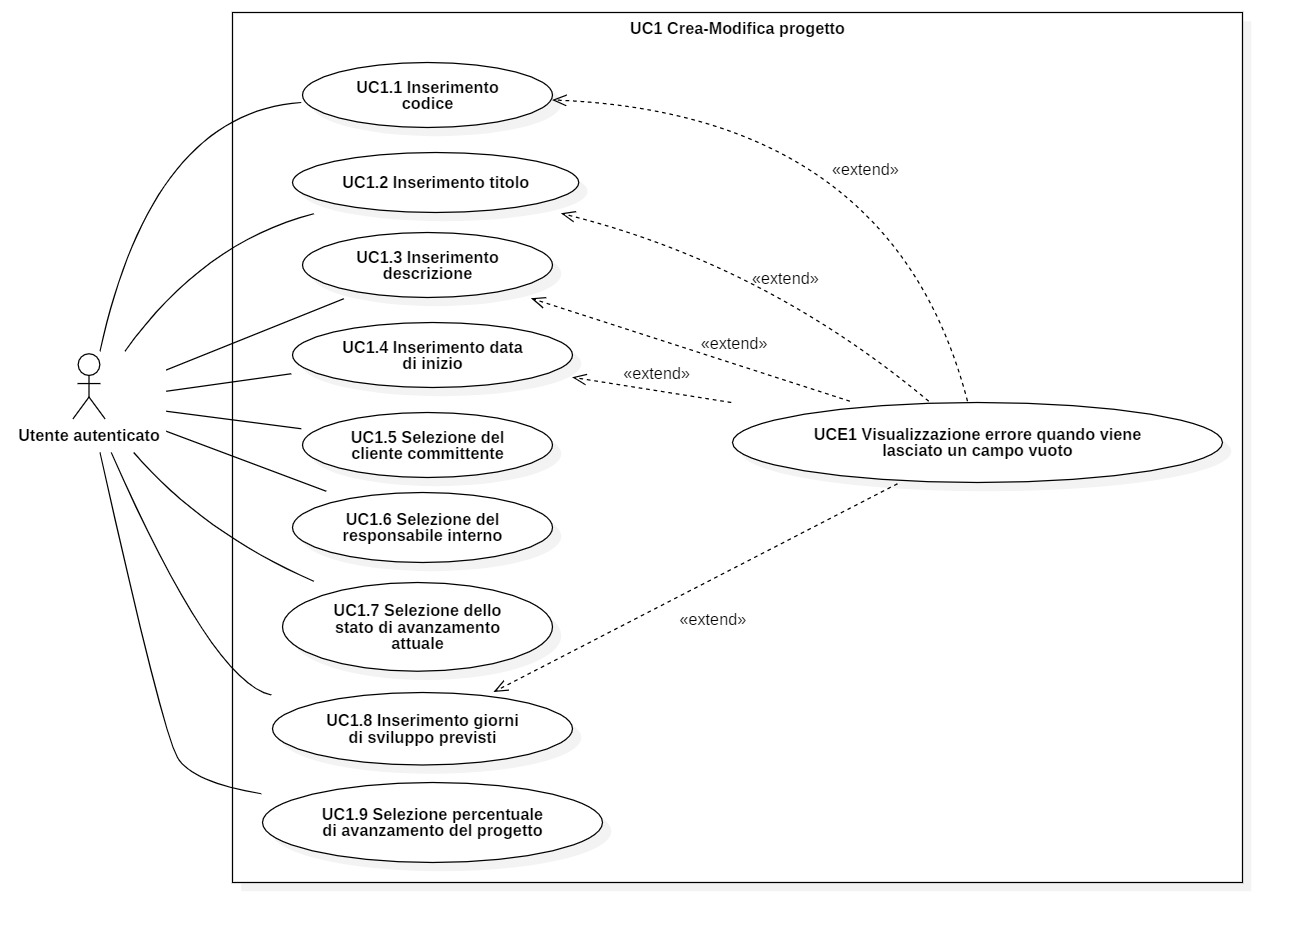
\includegraphics[width=400px]{../images/UC/.jpeg/UC1-nuovoModificaProgetto.jpg}
\caption{UC1: Crea-Modifica progetto}
\end{figure}

\begin{itemize}
\item \textbf{Attore primario}: Utente autenticato.
\item \textbf{Precondizione}: L'attore ha selezionato: 
\begin{itemize}
\item l'opzione \textit{nuovo progetto} dal menu;
\item l'opzione \textit{modifica} dal dettaglio di un progetto
\end{itemize}
\item \textbf{Postcondizione}: L'attore ha creato/modificato un progetto.
\item \textbf{Scenario principale}: 
\begin{enumerate}
\item L'attore inserisce/modifica il codice del progetto [UC1.1].
\item L'attore inserisce/modifica il titolo del progetto [UC1.2].
\item L'attore inserisce/modifica la descrizione del progetto [UC1.3].
\item L'attore inserisce/modifica la data di inizio del progetto [UC1.4].
\item L'attore seleziona/modifica il cliente committente [UC1.5].
\item L'attore seleziona/modifica il responsabile interno assegnato al progetto [UC1.6].
\item L'attore seleziona/modifica lo stato di avanzamento attuale delle attività [UC1.7].
\item L'attore inserisce/modifica i giorni di sviluppo previsti [UC1.8].
\item L'attore seleziona/modifica la percentuale di avanzamento delle attività di progetto [UC1.9].
\end{enumerate}
\item \textbf{Estensioni}: 
\begin{itemize}
\item L'attore visualizza un messaggio di errore quando viene lasciato un campo vuoto [UCE1].
\end{itemize} 
\end{itemize}

\pagebreak

\subsection{UC2: Tabella progetti}
\begin{figure}[!h]
\centering
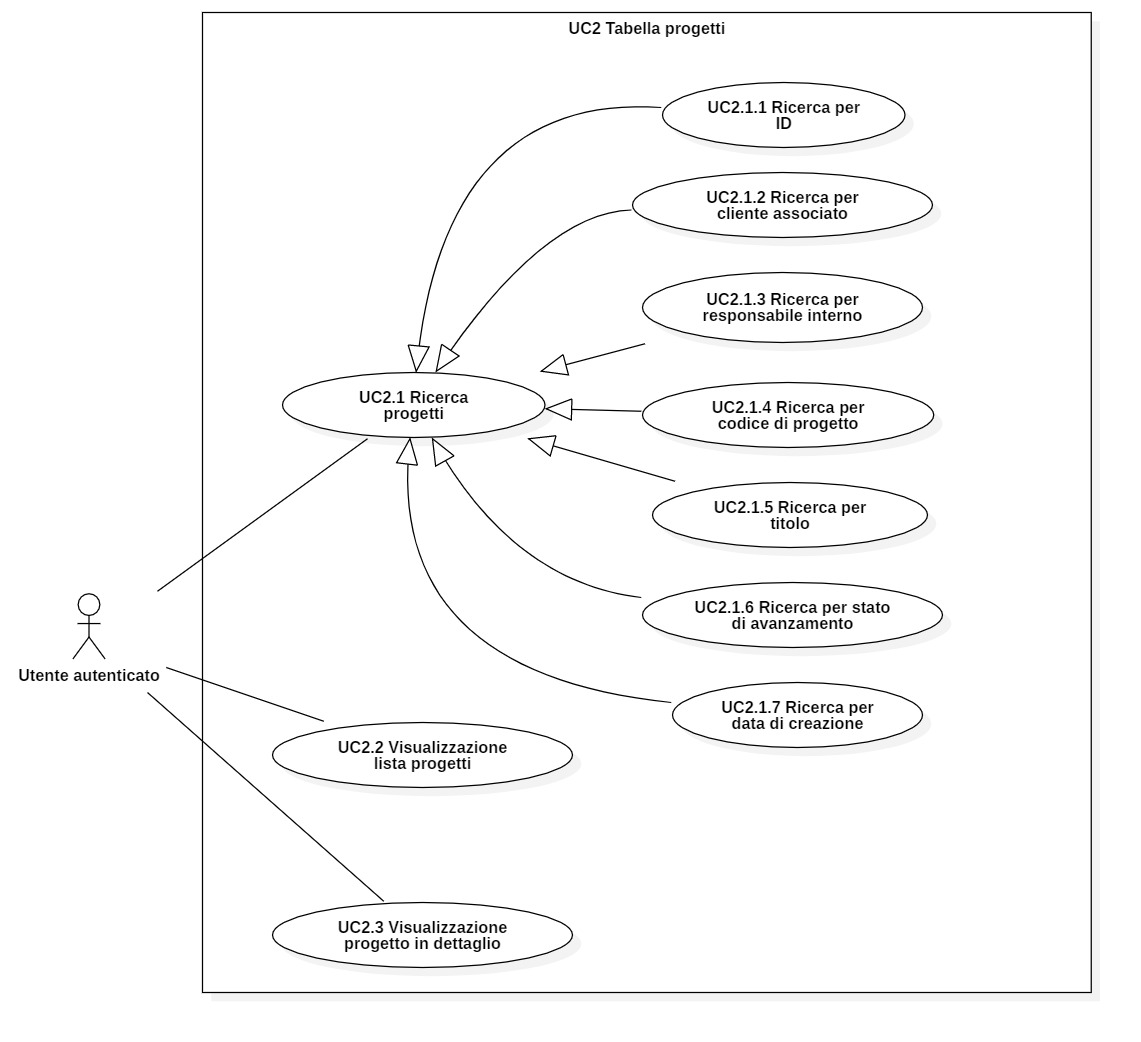
\includegraphics[width=300px]{../images/UC/.jpeg/UC2.0-tabellaProgetti.jpg}
\caption{UC2: Tabella progetti}
\end{figure}

\begin{itemize}
\item \textbf{Attore primario}: Utente autenticato.
\item \textbf{Precondizione}: L'attore ha selezionato l'opzione \textit{tabella progetti} dal menu.
\item \textbf{Postcondizione}: L'attore ha accesso alla tabella dei progetti.
\item \textbf{Scenario principale}: 
\begin{enumerate}
\item L'attore cerca uno o più progetti tramite la funzionalità di ricerca [UC2.1].
\item L'attore visualizza la lista completa dei progetti presenti nel sistema [UC2.2].
\item L'attore visualizza un progetto nel dettaglio [UC2.3].
\end{enumerate}
\end{itemize}

\pagebreak

\subsection{UC2.1: Ricerca progetti}
\begin{figure}[!h]
\centering
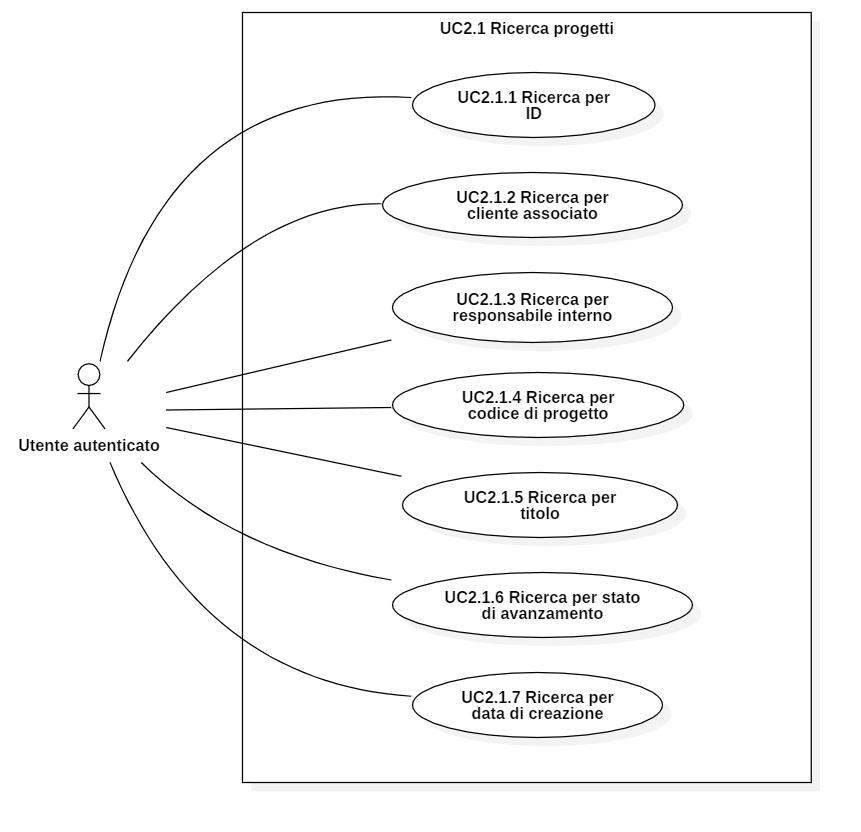
\includegraphics[width=300px]{../images/UC/.jpeg/UC2.1-ricercaProgetto.jpg}
\caption{UC2.1: Ricerca progetti}
\end{figure}

\begin{itemize}
\item \textbf{Attore primario}: Utente autenticato.
\item \textbf{Precondizione}: L'attore ha accesso alla tabella dei progetti.
\item \textbf{Postcondizione}: L'attore ha ricercato i progetti attraverso le opzioni di filtraggio disponibili.
\item \textbf{Scenario principale}: 
\begin{enumerate}
\item L'attore ricerca un progetto per ID [UC2.1.1].
\item L'attore ricerca un progetto per uno specifico cliente associato [UC2.1.2].
\item L'attore ricerca un progetto per responsabile interno [UC2.1.3].
\item L'attore ricerca un progetto per codice [UC2.1.4].
\item L'attore ricerca un progetto per titolo [UC2.1.5].
\item L'attore ricerca un progetto per stato di avanzamento [UC2.1.6].
\item L'attore ricerca un progetto per data di creazione [UC2.1.7].
\end{enumerate}
\end{itemize}

\pagebreak

\subsection{UC2.2: Visualizzazione lista progetti}
\begin{figure}[!h]
\centering
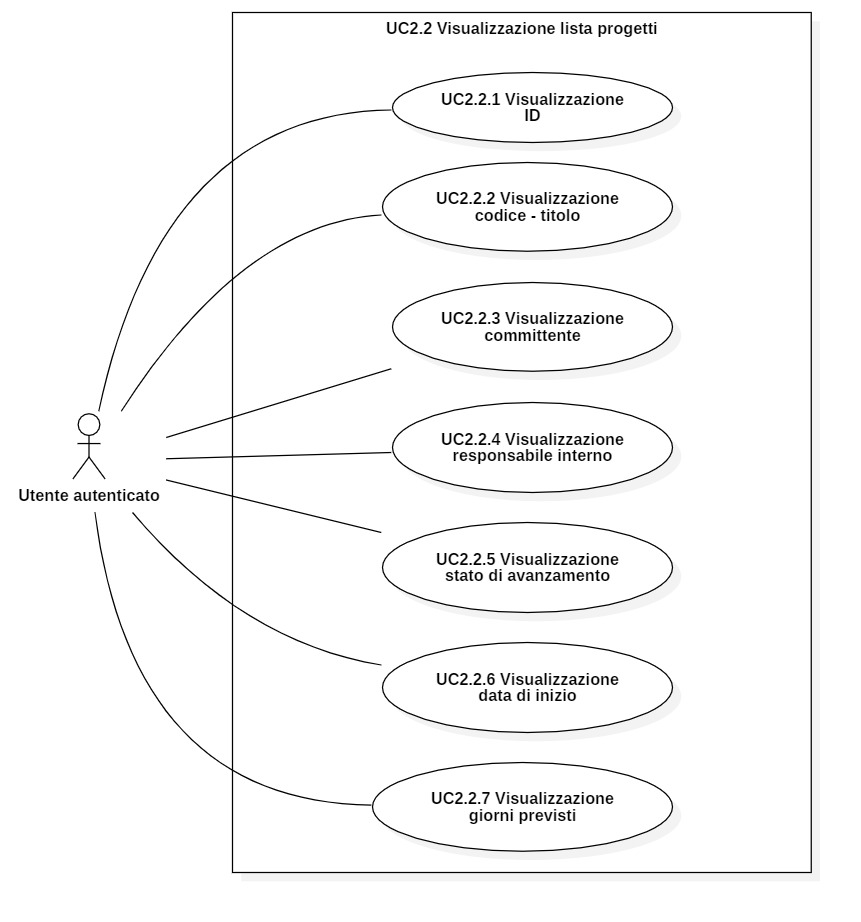
\includegraphics[width=300px]{../images/UC/.jpeg/UC2.2-visualizzazioneListaProgetti.jpg}
\caption{UC2.2: Visualizzazione lista progetti}
\end{figure}

\begin{itemize}
\item \textbf{Attore primario}: Utente autenticato.
\item \textbf{Precondizione}: L'attore ha accesso alla tabella dei progetti.
\item \textbf{Postcondizione}: L'attore ha visualizzato la lista dei progetti.
\item \textbf{Scenario principale}: 
\begin{enumerate}
\item L'attore visualizza l'ID del progetto [UC2.2.1].
\item L'attore visualizza la stringa "codice - titolo" del progetto [UC2.2.2].
\item L'attore visualizza il committente del progetto [UC2.2.3].
\item L'attore visualizza il responsabile interno del progetto [UC2.2.4].
\item L'attore visualizza lo stato di avanzamento del progetto [UC2.2.5].
\item L'attore visualizza la data di inizio del progetto [UC2.2.6].
\item L'attore visualizza i giorni di sviluppo previsti del progetto [UC2.2.7].
\end{enumerate}
\end{itemize}

\pagebreak

\subsection{UC2.3: Visualizzazione progetto in dettaglio}
\begin{figure}[!h]
\centering
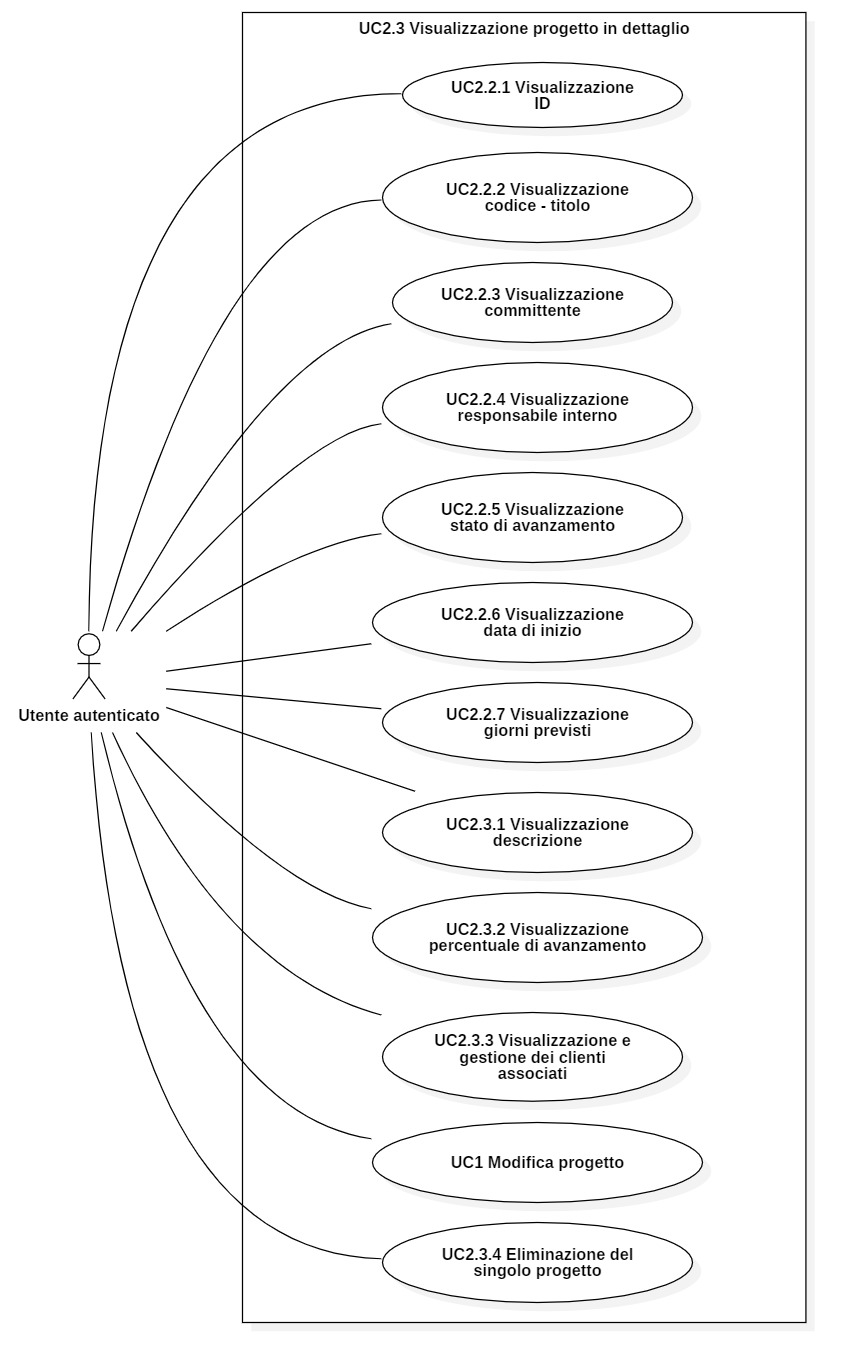
\includegraphics[width=300px]{../images/UC/.jpeg/UC2.3-visualizzazioneDettaglioProgetto.jpg}
\caption{UC2.3: Visualizzazione progetto in dettaglio}
\end{figure}

\begin{itemize}
\item \textbf{Attore primario}: Utente autenticato.
\item \textbf{Precondizione}: L'attore ha accesso alla tabella dei progetti.
\item \textbf{Postcondizione}: L'attore ha visualizzato il dettaglio di un progetto.
\item \textbf{Scenario principale}: 
\begin{enumerate}
\item L'attore visualizza l'ID del progetto [UC2.2.1].
\item L'attore visualizza la stringa "codice - titolo" del progetto [UC2.2.2].
\item L'attore visualizza il committente del progetto [UC2.2.3].
\item L'attore visualizza il responsabile interno del progetto [UC2.2.4].
\item L'attore visualizza lo stato di avanzamento del progetto [UC2.2.5].
\item L'attore visualizza la data di inizio del progetto [UC2.2.6].
\item L'attore visualizza i giorni di sviluppo previsti del progetto [UC2.2.7].
\item L'attore visualizza la descrizione del progetto [UC2.3.1].
\item L'attore visualizza la percentuale di avanzamento del progetto [UC2.3.2].
\item L'attore visualizza e gestisce i clienti associati al progetto [UC2.3.3].
\item L'attore può modificare il progetto [UC1].
\item L'attore può eliminare il progetto [UC2.3.4].
\end{enumerate}
\end{itemize}

\pagebreak

\subsection{UC3: Tabella progetti aperti}
\begin{figure}[!h]
\centering
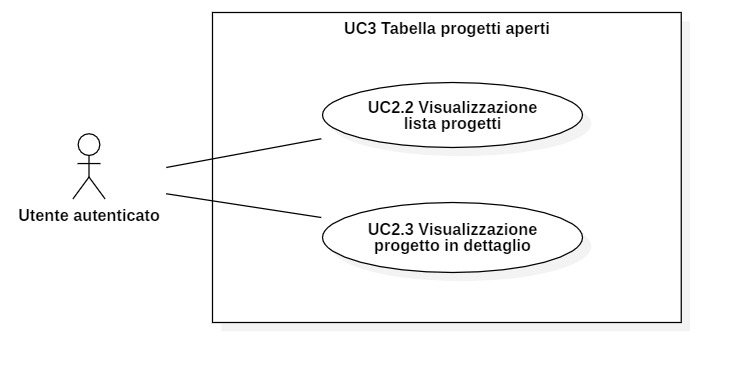
\includegraphics[width=300px]{../images/UC/.jpeg/UC3.0-tabellaProgettiAperti.jpg}
\caption{UC3: Tabella progetti aperti}
\end{figure}

\begin{itemize}
\item \textbf{Attore primario}: Utente autenticato.
\item \textbf{Precondizione}: L'attore ha selezionato l'opzione \textit{tabella progetti aperti} dal menu.
\item \textbf{Postcondizione}: L'attore ha accesso alla tabella dei progetti aperti.
\item \textbf{Scenario principale}: 
\begin{enumerate}
\item L'attore visualizza la lista dei progetti aperti presenti nel sistema [UC2.2].
\item L'attore visualizza un progetto aperto nel dettaglio [UC2.3].
\end{enumerate}
\end{itemize}

\pagebreak

\subsection{UC4: Tabella clienti}
\begin{figure}[!h]
\centering
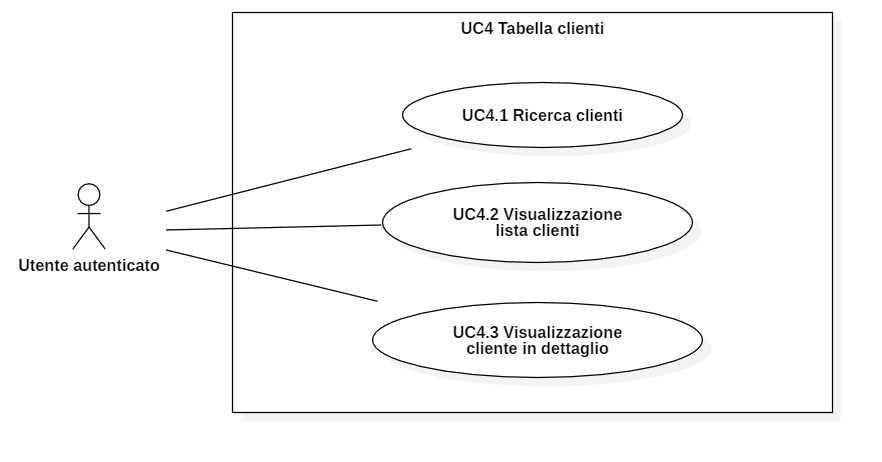
\includegraphics[width=300px]{../images/UC/.jpeg/UC4.0-tabellaClienti.jpg}
\caption{UC4: Tabella clienti}
\end{figure}

\begin{itemize}
\item \textbf{Attore primario}: Utente autenticato.
\item \textbf{Precondizione}: L'attore ha selezionato l'opzione \textit{tabella clienti} dal menu.
\item \textbf{Postcondizione}: L'attore ha accesso alla tabella dei clienti.
\item \textbf{Scenario principale}: 
\begin{enumerate}
\item L'attore cerca uno o più clienti tramite la funzionalità di ricerca [UC4.1].
\item L'attore visualizza la lista completa dei clienti presenti nel sistema [UC4.2].
\item L'attore visualizza un cliente nel dettaglio [UC4.3].
\end{enumerate}
\end{itemize}

\pagebreak

\subsection{UC4.1: Ricerca clienti}
\begin{figure}[!h]
\centering
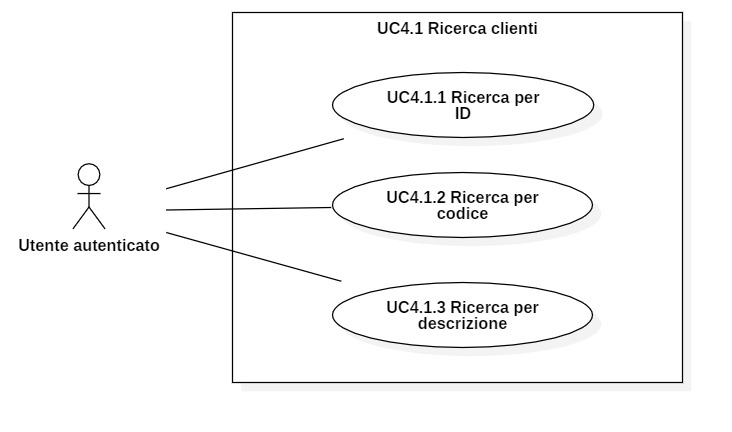
\includegraphics[width=300px]{../images/UC/.jpeg/UC4.1-ricercaCliente.jpg}
\caption{UC4.1: Ricerca clienti}
\end{figure}

\begin{itemize}
\item \textbf{Attore primario}: Utente autenticato.
\item \textbf{Precondizione}: L'attore ha accesso alla tabella dei clienti.
\item \textbf{Postcondizione}: L'attore ha ricercato i clienti attraverso le opzioni di filtraggio disponibili.
\item \textbf{Scenario principale}: 
\begin{enumerate}
\item L'attore ricerca un cliente per ID [UC4.1.1].
\item L'attore ricerca un cliente per codice (nominativo aziendale) [UC4.1.2].
\item L'attore ricerca un cliente per descrizione [UC4.1.3].
\end{enumerate}
\end{itemize}

\pagebreak

\subsection{UC4.2: Visualizzazione lista clienti}
\begin{figure}[!h]
\centering
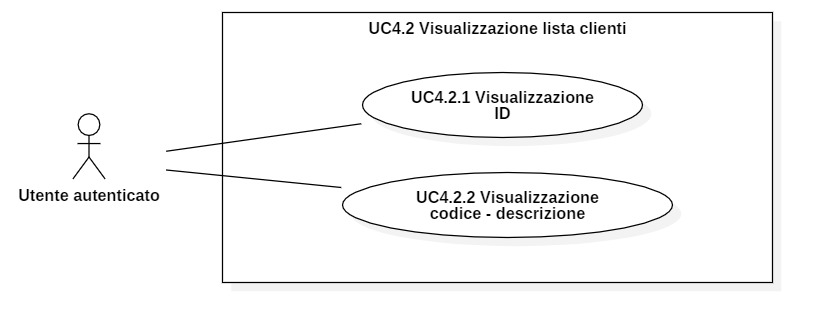
\includegraphics[width=300px]{../images/UC/.jpeg/UC4.2-visualizzazioneListaClienti.jpg}
\caption{UC4.2: Visualizzazione lista clienti}
\end{figure}

\begin{itemize}
\item \textbf{Attore primario}: Utente autenticato.
\item \textbf{Precondizione}: L'attore ha accesso alla tabella dei clienti.
\item \textbf{Postcondizione}: L'attore ha visualizzato la lista dei clienti.
\item \textbf{Scenario principale}: 
\begin{enumerate}
\item L'attore visualizza l'ID del cliente [UC4.2.1].
\item L'attore visualizza la stringa "codice - titolo" del cliente [UC4.2.2].
\end{enumerate}
\end{itemize}

\pagebreak

\subsection{UC4.3: Visualizzazione cliente in dettaglio}
\begin{figure}[!h]
\centering
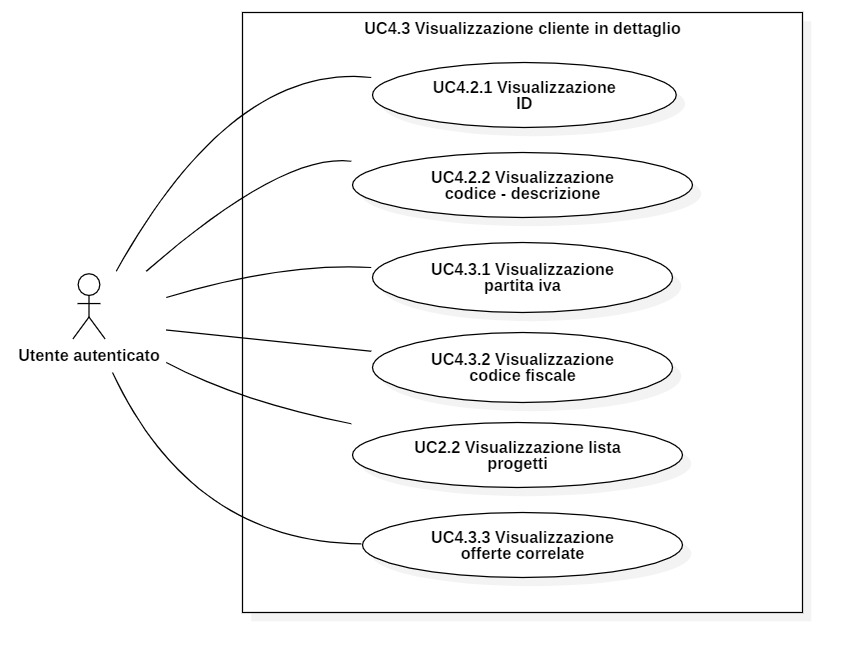
\includegraphics[width=300px]{../images/UC/.jpeg/UC4.3.0-visualizzazioneDettaglioCliente.jpg}
\caption{UC4.3: Visualizzazione cliente in dettaglio}
\end{figure}

\begin{itemize}
\item \textbf{Attore primario}: Utente autenticato.
\item \textbf{Precondizione}: L'attore ha accesso alla tabella dei clienti.
\item \textbf{Postcondizione}: L'attore ha visualizzato il dettaglio di un cliente.
\item \textbf{Scenario principale}: 
\begin{enumerate}
\item L'attore visualizza l'ID del cliente [UC4.2.1].
\item L'attore visualizza la stringa "codice - descrizione" del cliente [UC4.2.2].
\item L'attore visualizza la partita iva del cliente [UC4.3.1].
\item L'attore visualizza il codice fiscale del cliente [UC4.3.2].
\item L'attore visualizza la lista dei progetti associati al cliente [UC2.2].
\item L'attore visualizza le offerte correlate al cliente [UC4.3.3].
\end{enumerate}
\end{itemize}

\pagebreak

\subsection{UC4.3.3: Visualizzazione offerte correlate}
\begin{figure}[!h]
\centering
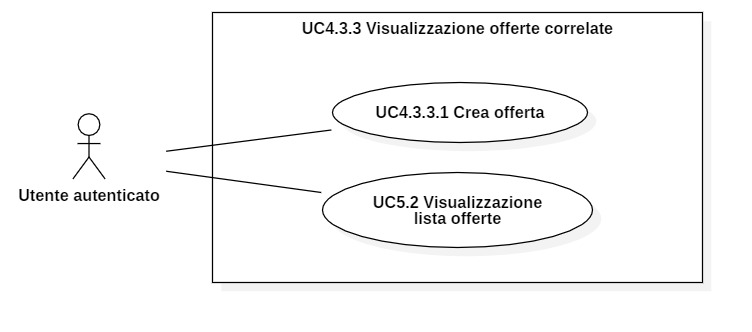
\includegraphics[width=300px]{../images/UC/.jpeg/UC4.3.3.0-visualizzazioneOfferteCorrelate.jpg}
\caption{UC4.3.3: Visualizzazione offerte correlate}
\end{figure}

\begin{itemize}
\item \textbf{Attore primario}: Utente autenticato.
\item \textbf{Precondizione}: L'attore ha visualizzato il dettaglio di un cliente.
\item \textbf{Postcondizione}: L'attore ha visualizzato le offerte correlate al cliente.
\item \textbf{Scenario principale}:
\begin{enumerate}
\item L'attore può creare una nuova offerta correlata al cliente [UC4.3.3.1].
\item L'attore visualizza la lista delle offerte del cliente [UC5.2].
\end{enumerate}
\end{itemize}

\pagebreak

\subsection{UC4.3.3.1: Crea-Modifica offerta}
\begin{figure}[!h]
\centering
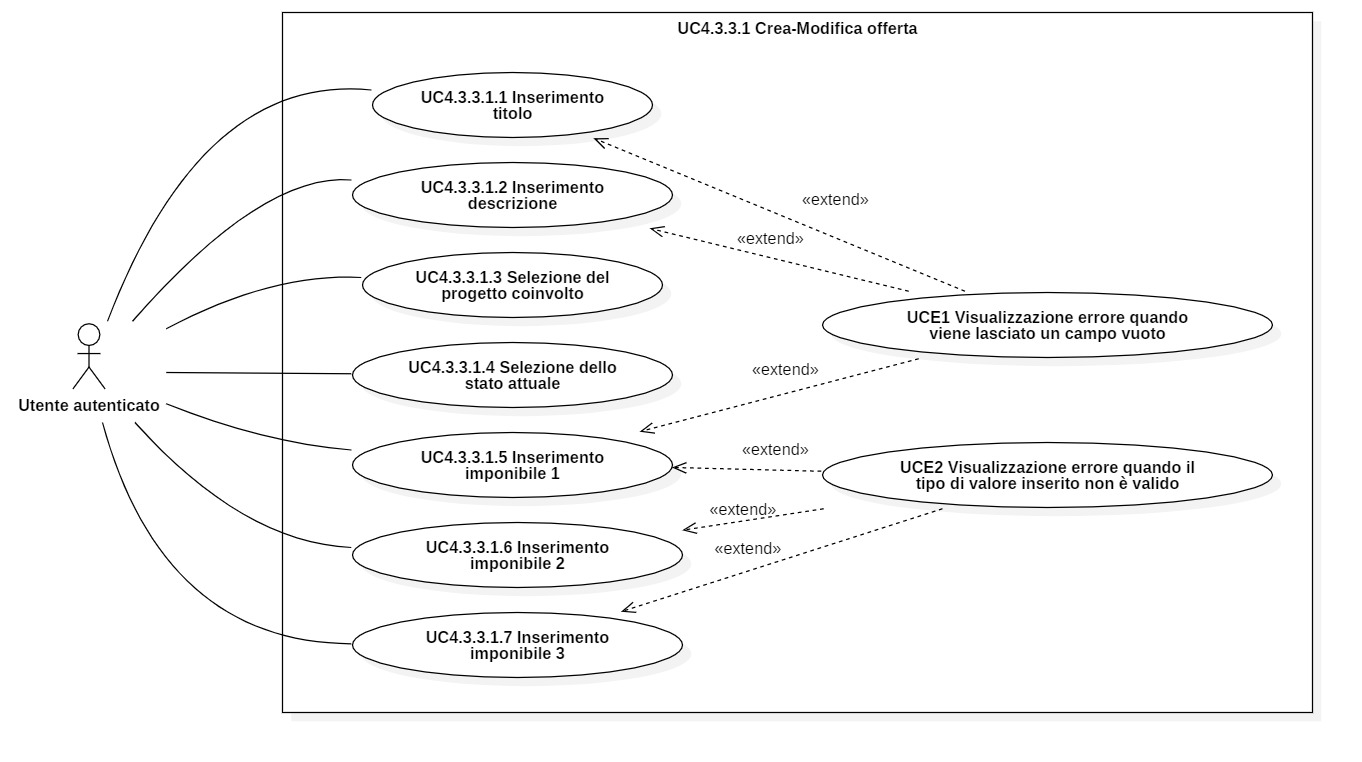
\includegraphics[width=400px]{../images/UC/.jpeg/UC4.3.3.1-nuovaModificaOfferta.jpg}
\caption{UC4.3.3.1: Crea-Modifica offerta}
\end{figure}

\begin{itemize}
\item \textbf{Attore primario}: Utente autenticato.
\item \textbf{Precondizione}: L'attore ha selezionato: 
\begin{itemize}
\item l'opzione \textit{nuova offerta} dal dettaglio di un cliente;
\item l'opzione \textit{modifica} dal dettaglio di un'offerta.
\end{itemize}
\item \textbf{Postcondizione}: L'attore ha creato/modificato un'offerta.
\item \textbf{Scenario principale}: 
\begin{enumerate}
\item L'attore inserisce/modifica il titolo di un'offerta [UC4.3.3.1.1].
\item L'attore inserisce/modifica la descrizione di un'offerta [UC4.3.3.1.2].
\item L'attore seleziona/modifica il progetto di riferimento di un'offerta [UC4.3.3.1.3].
\item L'attore seleziona/modifica lo stato attuale di un'offerta [UC4.3.3.1.4].
\item L'attore inserisce/modifica l'imponibile 1 di un'offerta [UC4.3.3.1.5].
\item L'attore inserisce/modifica l'imponibile 2 di un'offerta [UC4.3.3.1.6].
\item L'attore inserisce/modifica l'imponibile 3 di un'offerta [UC4.3.3.1.7].
\end{enumerate}
\item \textbf{Estensioni}: 
\begin{itemize}
\item L'attore visualizza un messaggio di errore quando viene lasciato un campo vuoto [UCE1].
\item L'attore visualizza un messaggio di errore quando viene inserito un tipo di valore non compatibile con quello del campo di interesse [UCE2].
\end{itemize} 
\end{itemize}

\pagebreak

\subsection{UC5: Tabella offerte}
\begin{figure}[!h]
\centering
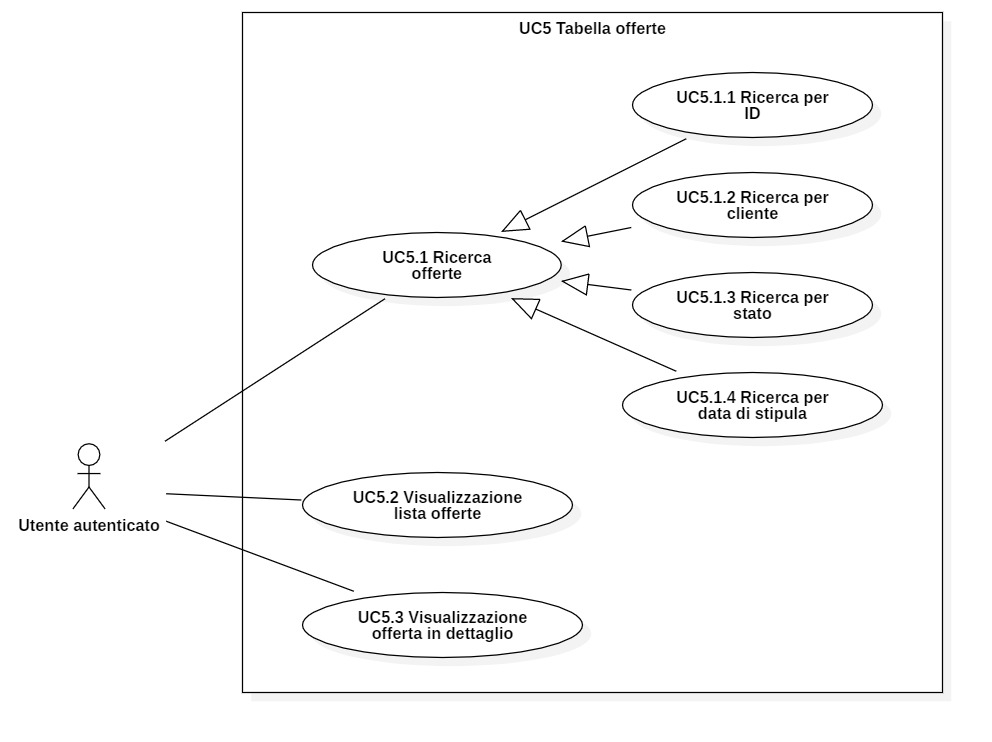
\includegraphics[width=300px]{../images/UC/.jpeg/UC5.0-tabellaOfferte.jpg}
\caption{UC5: Tabella offerte}
\end{figure}

\begin{itemize}
\item \textbf{Attore primario}: Utente autenticato.
\item \textbf{Precondizione}: L'attore ha selezionato l'opzione \textit{tabella offerte} dal menu.
\item \textbf{Postcondizione}: L'attore ha accesso alla tabella delle offerte.
\item \textbf{Scenario principale}: 
\begin{enumerate}
\item L'attore cerca una o più offerte tramite la funzionalità di ricerca [UC5.1].
\item L'attore visualizza la lista completa delle offerte presenti nel sistema [UC5.2].
\item L'attore visualizza un'offerta nel dettaglio [UC5.3].
\end{enumerate}
\end{itemize}

\pagebreak

\subsection{UC5.1: Ricerca offerte}
\begin{figure}[!h]
\centering
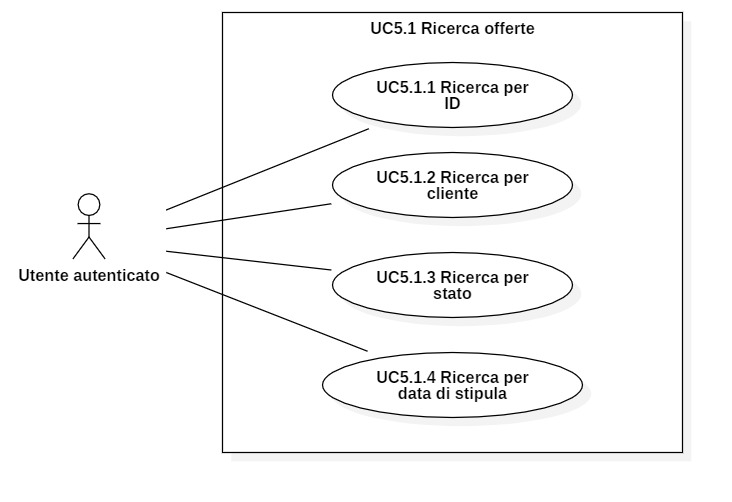
\includegraphics[width=300px]{../images/UC/.jpeg/UC5.1.0-ricercaOfferte.jpg}
\caption{UC5.1: Ricerca offerte}
\end{figure}

\begin{itemize}
\item \textbf{Attore primario}: Utente autenticato.
\item \textbf{Precondizione}: L'attore ha accesso alla tabella delle offerte.
\item \textbf{Postcondizione}: L'attore ha ricercato le offerte attraverso le opzioni di filtraggio disponibili.
\item \textbf{Scenario principale}: 
\begin{enumerate}
\item L'attore ricerca un'offerta per ID [UC5.1.1].
\item L'attore ricerca un'offerta per cliente associato [UC5.1.2].
\item L'attore ricerca un'offerta per stato attuale [UC5.1.3].
\item L'attore ricerca un'offerta per data di stipula [UC5.1.4].
\end{enumerate}
\end{itemize}

\pagebreak

\subsection{UC5.2: Visualizzazione lista offerte}
\begin{figure}[!h]
\centering
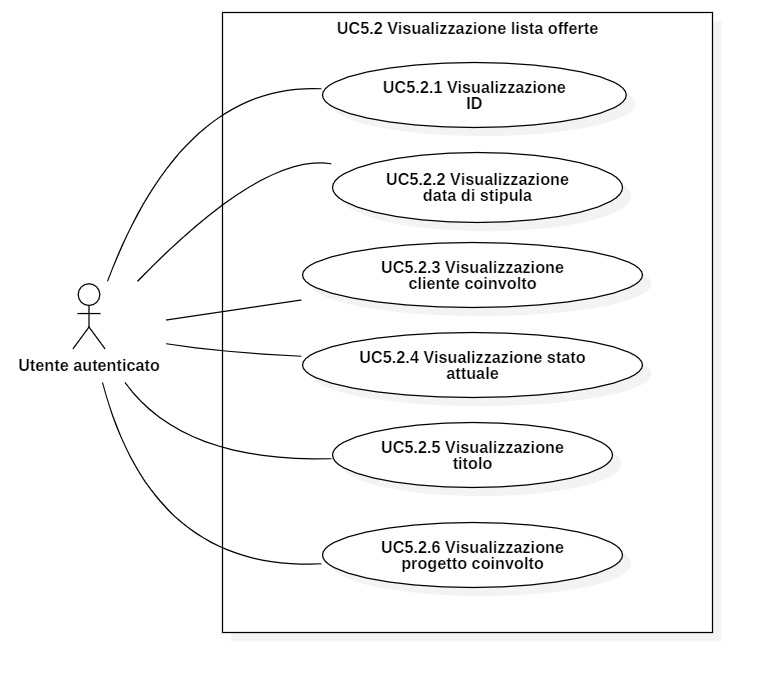
\includegraphics[width=300px]{../images/UC/.jpeg/UC5.2.0-visualizzazioneListaOfferte.jpg}
\caption{UC5.2: Visualizzazione lista offerte}
\end{figure}

\begin{itemize}
\item \textbf{Attore primario}: Utente autenticato.
\item \textbf{Precondizione}: L'attore ha accesso alla tabella delle offerte.
\item \textbf{Postcondizione}: L'attore ha visualizzato la lista delle offerte.
\item \textbf{Scenario principale}: 
\begin{enumerate}
\item L'attore visualizza l'ID dell'offerta [UC5.2.1].
\item L'attore visualizza la data di stipula dell'offerta [UC5.2.2].
\item L'attore visualizza il cliente coinvolto nell'offerta [UC5.2.3].
\item L'attore visualizza lo stato attuale dell'offerta [UC5.2.4].
\item L'attore visualizza il titolo dell'offerta [UC5.2.5].
\item L'attore visualizza il progetto coinvolto nell'offerta [UC5.2.6].
\end{enumerate}
\end{itemize}

\pagebreak

\subsection{UC5.3: Visualizzazione offerta in dettaglio}
\begin{figure}[!h]
\centering
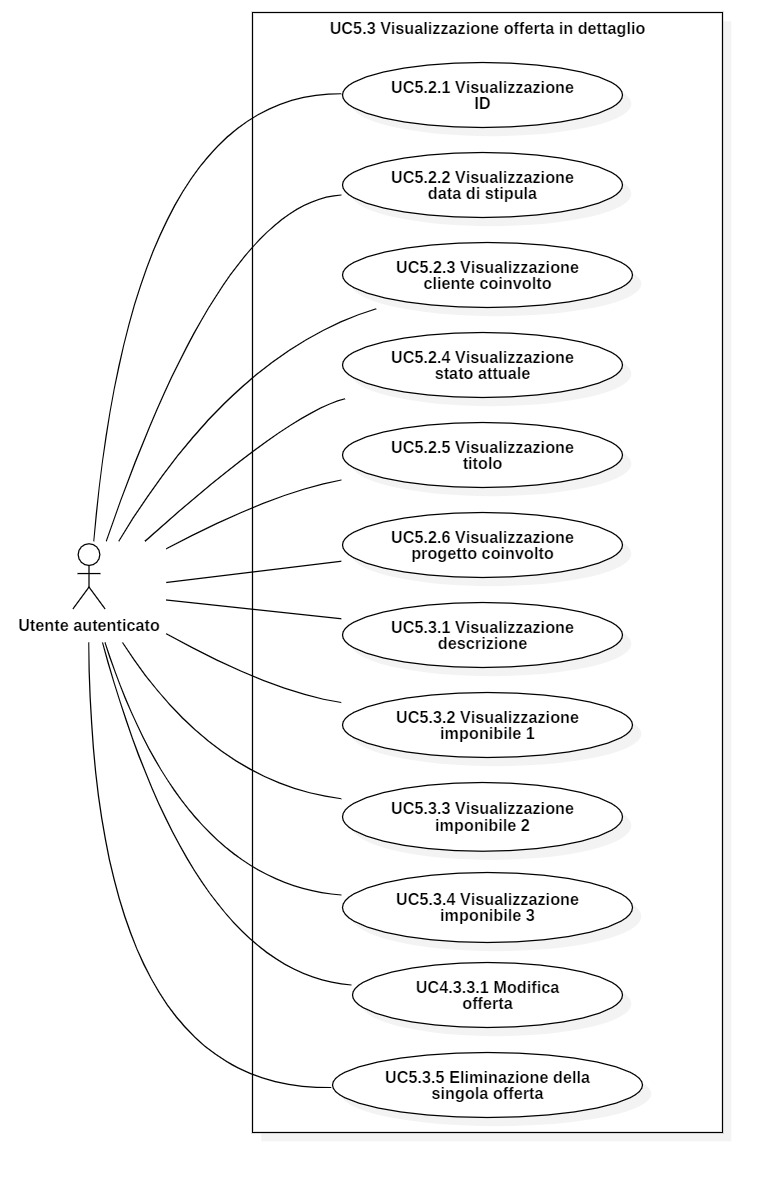
\includegraphics[width=300px]{../images/UC/.jpeg/UC5.3.0-visualizzazioneDettaglioOfferta.jpg}
\caption{UC5.3: Visualizzazione offerta in dettaglio}
\end{figure}

\begin{itemize}
\item \textbf{Attore primario}: Utente autenticato.
\item \textbf{Precondizione}: L'attore ha accesso alla tabella delle offerte.
\item \textbf{Postcondizione}: L'attore ha visualizzato il dettaglio di un'offerta.
\item \textbf{Scenario principale}: 
\begin{enumerate}
\item L'attore visualizza l'ID dell'offerta [UC5.2.1].
\item L'attore visualizza la data di stipula dell'offerta [UC5.2.2].
\item L'attore visualizza il cliente coinvolto nell'offerta [UC5.2.3].
\item L'attore visualizza lo stato attuale dell'offerta [UC5.2.4].
\item L'attore visualizza il titolo dell'offerta [UC5.2.5].
\item L'attore visualizza il progetto coinvolto nell'offerta [UC5.2.6].
\item L'attore visualizza la descrizione dell'offerta [UC5.3.1].
\item L'attore visualizza l'imponibile 1 dell'offerta [UC5.3.2].
\item L'attore visualizza l'imponibile 2 dell'offerta [UC5.3.3].
\item L'attore visualizza l'imponibile 3 dell'offerta [UC5.3.4].
\item L'attore può modificare l'offerta [UC4.3.3.1].
\item L'attore può eliminare l'offerta [UC5.3.5].
\end{enumerate}
\end{itemize}

\pagebreak

\section{Definizione e tracciamento dei requisiti}

